\section{Results \& Discussion - Qualitative Analysis}

Figure \ref{fig:DynamicClusterTimes} shows three different view of the same wake predicted by a simple Horseshoe Vortex.  It is a screen shot taken from the simulation running in Real-Time using 1024 elements arranged in a grid of 32x32 elements. The convective scheme used was the Dynamic Clustering scheme and the discretization method was the Quadratic Velocity scheme. The second to last row of elements on either side in the x-direction were given initial vorticity. Rows spanning the x-direction were spawned every $0.3s$. The spacing in the x-direction between consecutive elements was 0.5. The free-stream velocity of the flow was 0.5. 
\\\\
From figure \ref{fig:DynamicClusterTimes} a number of features are notable. Firstly wingtip vortices are present and the vortex sheet can be seen to roll up tightly at either side. Secondly the central portion of the sheet is seen to move downward in the vertical direction (a consequence of lift generation) under the influence of the horseshoe vortex. This is the shape that is expected to results from a horseshoe vortex. However, bumpiness along the vortex sheet can be seen in the central section, this is an error likely introduced by the way the location of clusters are calculated and was outlined in the discussion of the fixed cluster size scheme. However unique to this example is the presence of a bump with two bumps of relatively lower magnitude, this is likely caused by the addition of extra clustering abstractions.
\\\\
However, even with the presence of errors the vortex sheet is well formed and visually looks correct. However this says nothing of the simulations accuracy relative to experimental data. With the promising results obtained from the simulation though there is a definitely a case for pursuing further investigations into the accuracy of the simulation further.
\begin{figure}[H]
\centering
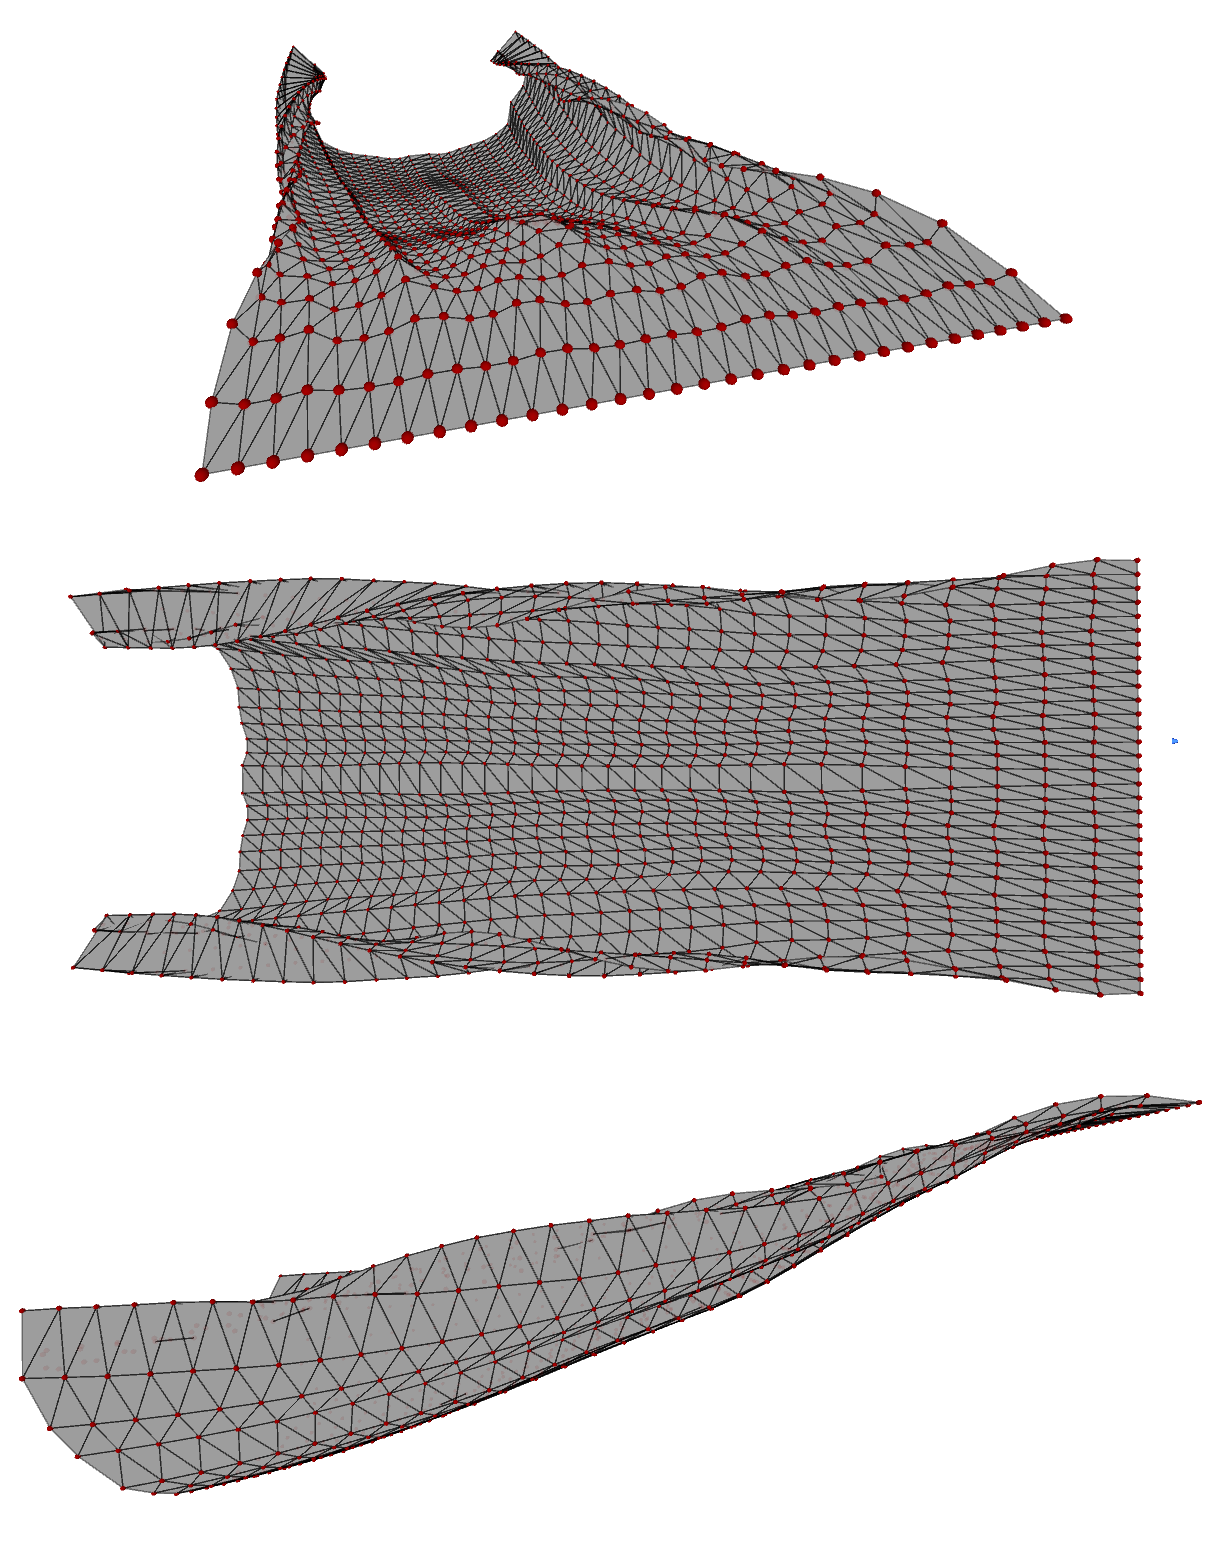
\includegraphics[width=1.0\textwidth]{Figures/HorseShoeVortexSheet.png}
\caption{\label{fig:DynamicClusterTimes} Increase in computational time given increased element count for the unoptimized case and dynamic cluster scaling}
\end{figure} 

